%============================================================================
\documentclass[a4paper, 11pt]{article}
\usepackage{comment} % enables the use of multi-line comments (\ifx \fi) 
\usepackage{lipsum} % generates Lorem Ipsum filler text. 
\usepackage{fullpage} % changes the margin
\usepackage{graphicx} % allows insertion of images
\graphicspath{ {../figures/} }
\usepackage{amsfonts}
\usepackage{amsmath}
\usepackage{subfig}
\usepackage{algpseudocode}
\usepackage{letltxmacro}
\LetLtxMacro{\oldalgorithmic}{\algorithmic}
\LetLtxMacro{\endoldalgorithmic}{\endalgorithmic}
\renewenvironment{algorithmic}[1][0]{%
  \hrulefill\par
  \oldalgorithmic[#1]}
  {\endoldalgorithmic\par
   \vspace*{-.5\baselineskip}
   \hrulefill\par
  }

\usepackage{listings}
\usepackage{color}
 
\definecolor{codegreen}{rgb}{0,0.6,0}
\definecolor{codegray}{rgb}{0.5,0.5,0.5}
\definecolor{codepurple}{rgb}{0.58,0,0.82}
\definecolor{backcolour}{rgb}{0.95,0.95,0.92}
 
\lstdefinestyle{mystyle}{
    backgroundcolor=\color{backcolour},   
    commentstyle=\color{codegreen},
    keywordstyle=\color{magenta},
    numberstyle=\tiny\color{codegray},
    stringstyle=\color{codepurple},
    basicstyle=\footnotesize\ttfamily,
    breakatwhitespace=false,         
    breaklines=true,                 
    captionpos=b,                    
    keepspaces=true,                 
    numbers=left,                    
    numbersep=5pt,                  
    showspaces=false,                
    showstringspaces=false,
    showtabs=false,                  
    tabsize=2
}
 
\lstset{style=mystyle}

% tight center environment
\newenvironment{tightcenter}{\setlength\topsep{0pt}\setlength\parskip{0pt}
  \begin{center}
}{%
  \end{center}
}

%Custom Commands
\newcommand{\hl}{\begin{center} \line(1,0){475} \end{center}} % lines
\newcommand{\ctitle}[1]{\begin{center} \LARGE{#1} \end{center}} % custom title
\newcounter{fignum} \stepcounter{fignum} % counter for figure captions
\newcommand{\ecap}[1]{\begin{tightcenter} Figure \arabic{fignum}: {#1} \end{tightcenter} \stepcounter{fignum}} % easy caption
%============================================================================

% EE 16B FINAL PROJECT REPORT TEMPLATE, SPRING 2018
%	Based on the ECE 100 template by Patrick Bartman.
%	Edited by Mia Mirkovic and Dinesh Parimi.
%
% INSTRUCTIONS: Replace all the \lipsum with your text and delete all <> and 
% examples/placeholders/fillers when finished. If you use external sources, 
% make sure to include them in the References section and cite them with the 
% \cite command as demonstrated. The rest should be self-explanatory. GLHF!

\begin{document}

%Header 
\noindent
Udacity Machine Learning Nano Degree \hfill Francesco Battocchio \\

%Title

\ctitle{Capstone Project Report: Learn to play Atari through Deep Reinforcement Learning}


\hl
\section{Definition}
\subsection{Project Overview}\label{sec:overview}
In reinforcement learning (RL) an agent interacts with an environment over a number of discrete time steps. At each time step the agent experiences a state $s$ of the environment and decides to perform an action $a$. The action to be performed in a particular state is defined by the policy $\pi(a|s)$, and the quality of the policy is expressed in terms of the return $R_t$ through the action-value function $Q^{\pi}(s,a) = \mathbb{E}[R_t|s_t=s, a]$. In Q-learning the learning task involves finding the optimal value function $Q^*(s,a)$, which leads to the maximum possible return. Once $Q^*(s,a)$ in known, the strategy is to act greedly with respect to $a$, or in other words to select at each step the action that maximise $Q^*(s,a)$.  If the state space is very large a function approximator, typically a neural network (NN), is used to model the optimal policy $Q^*(s,a) \approx Q(s,a,\theta)$. This type of learning agent, which is called deep Q-network (DQN), led to the first algorithm that outperformed humans in playing Atari \cite{Mnih2013}.\\
Nevertheless DQN can suffer from a problematic convergence and large training times. Convergence issued have been addressed through experience replay, and by adopting a separated target network to prevent training on correlated samples \cite{Mnih2015}. Still, this solution does not guarantee good performances in all the different RL problems. More recently policy gradient (PG) methods have been revived as they have shown for some applications superior converge while reducing training time compared to DQN \cite{Mnih2016}. In this class of algorithms a NN is used to approximate the policy that maximises the expected reward $\pi^*(a|s) \approx \pi(s,a,\mathbf{\theta})$. Policy parameters learning is based on the gradient of the performance measure with respect to the policy parameters. PG methods however also do not work well universally and may require long time to find the correct hyperparameters. Perhaps the simplest advantage that policy parameterization may have over action-value is that the policy may be a simpler function to approximate compared to the action-value function. In fact, problems can have different complexity for their policies or action-value functions. For some, the action-value function is simpler and thus easier to approximate. For others, the policy is simpler. In the latter case a policy-based method will typically learn faster and yield a superior asymptotic policy \cite{Sutton}.  

\subsection{Problem Statement}
The aim of this project is to train a RL agent to play the Atari 2600 game Pong \cite{OpenAI} through two different reinforcement learning approaches described in Section \ref{sec:overview}. In Pong an agent and his opponent control a paddle, and the game consists of bouncing a ball past the other player. At each time step the agent observes a pixel image and chooses between two actions, Up or Down, then he receives a reward based on whether or not the ball went past the opponent. The reward is +1 if the ball went past the opponent, -1 if it went past the agent. In the original DeepMind implementation \cite{Mnih2013,Mnih2016} the states consist of the last 4 $84 \times 84$ pixels frames observed by the agent, which results on $256^{84 \times 84 \times 4} \approx 1.4 \times 10^{67970}$ different combinations. In such a large state space the state-value function $Q^{\pi}(s,a) $ or the policy  $\pi(s,a)$ cannot the stored in a table, but needs to be approximated by a NN. Such NN often requires several layers to beat the opponent consistently, which is the reason why this approach is called deep reinforcement learning.

\subsection{Metrics}
Each Pong episode is made of multiple consecutive games, and it finishes when one of the opponent reaches a score of 21. An agent who is not able to learn, or select actions at random, will lose the game most of the time. As a result, the return, i.e. the sum rewards at the end of an episode, will be always near to the minimum of -21. When the agent learns the action-value function, or the policy, it will start to outperform the opponent for an increasing number of games and the return will increase accordingly. Deep RL algorithms require in general very long training times to be able to beat consistently the agent, and are in general run on GPUs to speed up the calculations. The outstanding results in \cite{Mnih2016} where achieved after playing 10 millions episode, which translates into weeks of computational time. However, all the analyses in this project were run on a MacBook CPU 2.8 GHz 8 GB RAM. Since the scope of this project is to evaluate the performance of different algorithms, and not to outperform consistently the opponent, the training was limited to 2000 episodes. Therefore the performance of an algorithm is based on the evolution of the return along 2000 episodes played.
\hl

\section{Analysis}
\subsection{Data Exploration and Visualisation}\label{sec:data-exploration}
In a reinforcement learning problem the agent is not trained on a labelled data set, as in supervised learning, but instead he is required to understand the quality of his actions based on the rewards that he receives from the environment. In this project OpenAI Gym is used to replicate Atari 2600 Pong environment \cite{OpenAI}. Each input is an RGB image as shown in Figure \ref{fig:pong-frame}, which corresponds to an array of shape (210, 160,3), and the environment returns a reward of +1 if the ball went past the opponents, -1 if the ball is missed, or 0 otherwise.\\
The agent can choose between 6 discrete actions labelled from 0 to 6, in which (0,1) are idle actions that don't have any affect, (2,4) make the paddle go up, and (3,5) make the paddle go down \cite{PongActions}. Once an actions is selected it is repeatedly performed for a duration of $k$ frames, where $k$ is uniformly sampled from {2,3,4}. This introduces some degree of randomness in the agent behaviour, as the same policy leads to slightly different agent behaviours when repeated in different episodes.

% Pong frame
\begin{figure}[!htb]
  \begin{center}
   \includegraphics[height=0.25\textheight]{Pong_raw.jpeg}
    \caption{Pong frame.}
    \label{fig:pong-frame}
  \end{center}
\end{figure}  

\subsection{Algorithm and Techniques}
\subsubsection{DQN}
The DQN algorithm has been introduced by the Google Deepmind paper in 2015 \cite{Mnih2015}. A DNN is used to approximate the optimal action-value function:
\begin{equation}
Q^*(s,a) = \max_{\pi}\mathbb{E}\left[ r_t +\gamma r_{t+1} +\gamma^2 r_{t+2} + \dots \gamma^{T-t}r_T | s, a, \pi\right]
\end{equation}
which corresponds to the maximum expected return that can be achieved at any point in time following the policy $\pi$, under the hypothesis of discounted future rewards perametrised by $\gamma <1$. The optimal action-value function can be found iteratively from the Bellman equation, which states that if $Q^*(s',a')$ was known at the next state $s'$ for all actions $a'$, then the optimal greedy strategy is to select the action $a'$ that maximizes the expected value of $r+Q^*(s',a')$: 
\begin{equation}\label{eq:BellmanEq}
Q^*(s,a) = r +\gamma \max_{a'}Q^*(s',a')
\end{equation}
An action is selected according to an $\epsilon$-greedy strategy in which the greedy policy is followed with 1-$\epsilon$ probability, while a random action is selected with $\epsilon$ probability. 
A NN approximator of the optimal action value-function $Q^*(s,a) \approx Q(s,a,\theta)$ is trained on target values $y_i=r+\max_{a'} Q(s,a,\theta_{i-1})$ by defining a loss function:
\begin{equation}\label{eq:DQN-loss}
L(\theta_i) = \left( y_i - Q(s,a,\theta_{i}) \right)^2
\end{equation}
this means that the NN is updated using as target values its own outcomes obtained with current weights $\theta_{i+1}$, which are held fixed during the training step. Although this approach is proven to converge as $t\to\infty$, in practice it is observed that correlation that between $Q(s,a,\theta_{i})$ and the target value represents an issue. For this reason a strategy called \emph{experience replay} is adopted in which the observed transitions $(s_t, a_t, r_t, s_{t+1})$ are stored into a memory $D$. The weight update is then performed at the end of each episode on a random batch of transitions sampled from $D$. A summary of the DQN algorithm is shown in Figure \ref{fig:DQN_algorithm}  

\begin{figure}[!htb]
  \begin{algorithmic}
    \State Initialise action-value function parametrization $Q(s,a,\boldsymbol{\theta})$ with random weights $\boldsymbol{\theta}$
    \State Initialise memory $D$
    	\For{$episode = 1, \ldots, N$}
    		\Repeat
    			\State Observe state $s_t$ and perform action according to $\varepsilon$-greedy scheme
    			\State Observe episode rewad $r_t$ and next state $s_{t+1} $ 
    			\State Store transition $(s_t, a_t, r_t, s_{t+1})$ into $D$
    			\State Sample random mini-batch of transitions $(s_k , a_k, r_k, s_{k+1})$ from $D$
    			\If {$s_{t+1}$ is terminal}
    				\State $y_k = r_k$
    			\Else
    				\State $y_k = r_k + \gamma \max_{a'}(Q(s_{t+1}, a', \boldsymbol{\theta})$
    			\EndIf
    			\State Perform gradient descent $\boldsymbol{\theta} \gets \boldsymbol{\theta} + \alpha(y_k - Q(s,a,\boldsymbol{\theta})) \nabla Q(s,a,\boldsymbol{\theta})$
    		\Until{episode is finished}
    	\EndFor
  \end{algorithmic}
    \caption{DQN algorithm}\label{fig:DQN_algorithm}
\end{figure}

\subsubsection{Policy Gradient}
Policy gradient refers to a class of algorithms that originate from 1992 Williams' REINFORCE algorithm \cite{Williams1992}. Policy gradient method approximates the optimal policy $\pi^*(a|s) \approx \pi(s,a,\mathbf{\theta})$, instead of the action-value function $Q(s,a)$ used in DQN, and uses an unbiased estimate of the policy gradient to perform the weight update. Given the objective function $J(\mathbf{\theta}) = V_{\pi_{\theta}}(s_0)$ that measures the quality of policy $\pi_{\theta}$, the unbiased estimate of its gradient is given by \cite{Sutton}
\begin{equation}\label{eq:policy-gradient}
\nabla J(\mathbf{\theta})  =  \mathbb{E}\left[ R_t \nabla_\mathbf{\theta}\log \pi(s,a,\mathbf{\theta}\right]
\end{equation}  
which is used to perform the weight update by gradient ascent, since now we want to maximise $J(\mathbf{\theta})$.\\
In this work the basic implementation by Andrej Karpathy \cite{Karpathy} and described in Figure \ref{fig:PG_algorithm} will be used. A pre-defined number of episodes are played and stored in memory, and a discounted total reward is computed for each observed transition
\begin{equation}
r_{d,t} = \sum_{k=0}^{\infty} \gamma^k r_{t+k}
\end{equation}
the discounted rewards are normalised, and weight update is performed on the batch of samples currently stored in memory

\begin{figure}[!htb]
  \begin{algorithmic}
    \State Initialise policy parametrization $\pi(s,a,\boldsymbol{\theta})$ with random weights $\boldsymbol{\theta}$
    \State Initialise batch memory $D$
    	\For{$episode = 1, \ldots, N$}
    		\Repeat
    			\State Observe state $s_t$ and perform action $a_t \sim$ $\pi(s,a,\mathbf{\theta})$
    			\State Observe reward $r_t $ and compute discounted reward $r_{d,t}$
    			\State Store $(s_t, a_t, r_{d,t})$ into $D$
    		\Until{episode is finished}
    		\If {$episode \bmod batch \, size = 0$}
    			\State Perform weight update $\boldsymbol{\theta} \gets \boldsymbol{\theta} + \alpha r_{d,t} \nabla \ln \pi(s_t,a_t,\mathbf{\theta})$
    			\State Empty $D$
    		\EndIf
    	\EndFor
  \end{algorithmic}
    \caption{Policy gradient algorithm}\label{fig:PG_algorithm}
\end{figure}

\subsection{Benchmark}
The benchmark used to evaluate the performance of an algorithm is represented by the performance of an agent that selects actions uniformly at random. Figure \ref{fig:random-agent} shows that the moving average of the return remains between -21 and -20, that is the opponent is consistently winning most the games in an episode and the performance of the agent is not improving. It is expected that a \emph{learning} agent starts initially with similar performance to the random agent, but that he will improve with the number of games played.
% Random agent
\begin{figure}[!htb]
  \begin{center}
   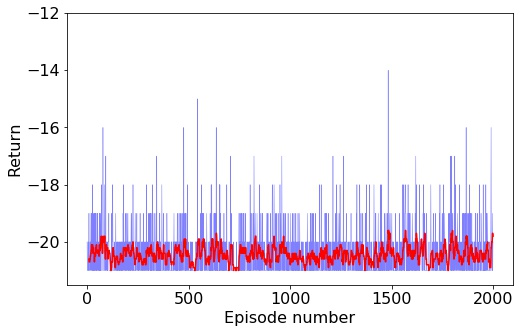
\includegraphics[width=0.4\textheight]{random_return.jpeg}
    \caption{Performance of a random agent, in blue the episode return and in red the moving average on a window of 10 episodes.}
    \label{fig:random-agent}
  \end{center}
\end{figure}  

\hl

\section{Methodology}
\subsection{Data preprocessing}
Figure \ref{fig:preprocessing-original} suggests that only the portion of the image between the two grey bands is needed to learn the game, and that colors do not contain any valuable informations. Therefore, a function is defined to pre-process the frames, which crops the central part of the frame and convert the image to a binary array with 0 assigned to the background and 1 to both the ball and the paddles. In addition, the image resolution is such that the geometries are preserved if the pixels are down-sampled by a factor of 2. The resulting frame which is shown in Figure \ref{fig:preprocessing-binary} contains the same amount of information as the original one, but reduces the complexity of the NN used by the learning agent.\\
A learning agent needs information of the current state as well as the previous ones in order to improve his performance. This because the correct action can be choosen only if the trajectory of the ball is known or, in other words, if both velocity and position are available. In the DQN implementation of Google Deepmind \cite{Mnih2015} the authors have used a stack of the 4 previous images as current state. This solution leads to a computationally expensive model which was well suited for their CNN architecture. A simplified solution, which has been introduced in \cite{Karpathy}, and is widely adopted for testing codes, is to let the agent observe the difference between the current and the previous frame. The difference image which is shown in Figure \ref{fig:preprocessing-difference} indicates that the opponent (on the left) has moved downward, the player (on the right) has moved upward, and the ball is going towards the opponent.\\
In Section \ref{sec:data-exploration} it was observed that out of the 6 actions that the agent can perform in the Pong OpenAI version, only 2 are needed to play a game. This allows to simplify the output of the NN into a binary index (0,1) that maps to action label 2 to move the paddle up, and action label 3 to move the paddle down. Although this is not expect to reduce the computational complexity it allow to simplify the code.
%Frame preprocessing
 \begin{figure}[!htb]
  \begin{center}
  	\subfloat[]{
   		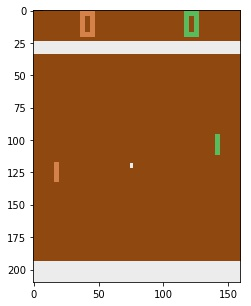
\includegraphics[width=0.2\textheight]{pong_raw.jpeg}\label{fig:preprocessing-original}}
 	\subfloat[]{
   		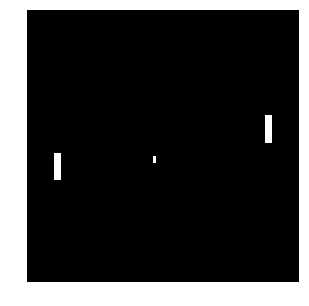
\includegraphics[width=0.2\textheight]{pong_processed.jpeg}\label{fig:preprocessing-binary}}
   	\subfloat[]{
   		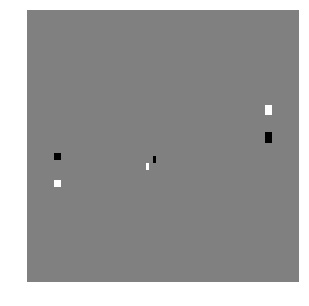
\includegraphics[width=0.2\textheight]{pong_difference.jpeg}\label{fig:preprocessing-difference}}
    \caption{Frame preprocessing: (a) current original frame, (b) binary image after cropping and down-sampling, and (c) difference between next frame and current frame.}
    \label{fig:Preprocessing}
  \end{center}
\end{figure}

\subsection{Implementation}
Following a similar approach to \cite{Jaromiru} a RL algorithm is organised into 3 Python classes: 
\begin{itemize}
\item the \texttt{Agent} who performs actions, observes the environment, and learns from the feedback of the environment;
\item the agent's \texttt{Brain} which contains the definition of the NN architecture, training, prediction, and weight update procedures
\item the \texttt{Environment} in which the agent learns, which returns the new state and the reward that follow an agent action in a loop that repeat for a large number of episodes
\end{itemize}
The initial NN architecture tested for both the DQN and the PG methods was the same as in \cite{Mnih2013} composed of 2 convolutional layers and a fully connected layer, and used as inputs stacks of 2 consecutive frames (insted of 4 frames as in the original paper). This configuration however required very large computational times which posed limitations to the testing and development of the codes. For this reason the same simplified network architecture in \cite{Karpathy}  was adopted for both the DQN and the Policy Gradient algorithm which consisted of a single fully connected hidden layer of 200 units. The algorithms which are described in detail in the next section were  implemented using \emph{Keras} and \emph{Tensorflow} Python libraries. 

\subsubsection{DQN algorithm}
The \texttt{Agent} class stores samples into the memory, update the $\epsilon$ parameter, maps the NN outputs to the action label, and implements the \texttt{replay} function which calculates the NN target using Equation \ref{eq:BellmanEq} and performs the network weight update. The target network is used to assign to the agent network the target Q-value ($y_i$ in Equation \ref{eq:DQN-loss}) for the current action. A more efficient implementation which use a single network to perform the learning step \cite{Ecoffet}, was also tested but this didn't reduce significantly the training time.
\begin{lstlisting}[language=Python, caption=DQN Agent definition, label={lst:DQN-agent}]
class Agent:
    def __init__(self, stateCnt, actionCnt):
        self.stateCnt = stateCnt
        self.actionCnt = actionCnt
        self.memory = deque(maxlen = REPLAY_MEMORY) 
        self.brain = Brain(stateCnt, actionCnt)
        
    def action_index(self, s):
        """ Select action index action according to epsilon-greedy scheme """
        if random.random() < self.epsilon:
            index = random.randint(0, self.actionCnt-1)
        else:
            index = np.argmax(self.brain.predictOne(s))
        return index
  
    def observe(self, sample):
        """ Add sample to memory, decrease epsilon, update target network"""
        self.memory.append(sample)
        self.steps += 1
        if self.epsilon > FINAL_EPSILON:
            self.epsilon -= (INITIAL_EPSILON - FINAL_EPSILON) / EXPLORATION
        # update target network 
        if self.steps % UPDATE_TARGET_FREQUENCY == 0:
            self.brain.updateTargetModel()
    
    
    def replay(self):
        """ Sample experience from memory and update weights """
        if len(self.memory) < BATCH_SIZE: 
            return        
        # sample from memory queue
        batch = np.array(random.sample(self.memory, BATCH_SIZE))    
        states = np.vstack(batch[:,0])
        actions_index = np.vstack(batch[:,1])
        rewards = np.vstack(batch[:,2])
        next_states = np.vstack(batch[:,3])
        terminals = np.vstack(batch[:,4])
        
        # current state predictions from AGENT network
        Q = self.brain.predict(states)
        # next_state predictions from TARGET network
        next_Q = self.brain.predict(next_states, target=True)
        # target Q values - if terminal: target_Q = rewards
        target_Q = rewards + GAMMA * np.max(next_Q, axis=1) * np.invert(terminals)
        # assign target values to actions
        Q[range(BATCH_SIZE), actions_index] = target_Q 
        # AGENT network update
        self.brain.train(states, Q)
        self.Q_sa = next_Q
\end{lstlisting}

The \texttt{Brain} class defines the NN model of the action-value function $Q(s,a,\theta)$ implemented in \emph{Keras}, which uses a RMSprop optimizer and a custom Huber loss function to clip the gradient \cite{Ecoffet}. The output of the network is a binary array (0,1) which is then used to select the paddle actions Up and Down.  
\begin{lstlisting}[language=Python, caption=DQN Brain definition, label={lst:DQN-brain}]
class Brain:
    def __init__(self, stateCnt, actionCnt):
        self.stateCnt = stateCnt
        self.actionCnt = actionCnt      
        self.model = self._createModel()
        self.model_ = self._createModel()  # target model
   
    def _createModel(self):
        """ Implement NN to approximate action-value function Q(s,a)=Q(s,a,w) 
        """
        model = Sequential()
        model.add(Dense(output_dim=200, activation='relu', input_dim=self.stateCnt))
        model.add(Dense(output_dim=actionCnt, activation='linear'))
        
        opt = RMSprop(lr=LEARNING_RATE, decay=DECAY_RATE)
        model.compile(loss=huber_loss, optimizer=opt)        
        return model
    
    def train(self, x, y, epochs=1):
        """ Trains the model for a fixed number of epochs """
        self.model.fit(x, y, batch_size=BATCH_SIZE, epochs=epochs, verbose=0)
        
    def predict(self, s, target=False):
        """ Batch prediction from agent network or target network """
        if target:
            return self.model_.predict(s)
        else:
            return self.model.predict(s)
    
    def predictOne(self, s, target=False):
        """ Predict one action from model """
        return self.predict(s.reshape(1, self.stateCnt), target=target).flatten()
    
    def updateTargetModel(self):
        """assign weights to target Network """
        self.model_.set_weights(self.model.get_weights())
\end{lstlisting}

The \texttt{Environment} class implements the DQN algorithm shown in Figure \ref{fig:DQN_algorithm} in which the agent observes a state, represented by the difference between the current and the previous frame, performs an action and observes the new state and reward. Then a transition is stored in memory and the network weight update is performed through the \texttt{replay} function at the end of each step. 
\begin{lstlisting}[language=Python, caption=DQN Environment definition, label={lst:DQN-environment}]
class Environment():    
    def __init__(self, game):
        self.game = game
        self.env = gym.make(game)
        
    def run(self, agent):
        """ DQN algorithm """
        obs = self.env.reset()
        prev_image = preprocess(obs)
        state = np.zeros(stateCnt)
        R = 0       
        while True:       
            # agent performs action: labels:(0,1) -> actions:(2,3)
            action_index = agent.action_index(state)
            action = action_index+2
            # environment return new state and reward
            obs, reward, done, _ = self.env.step(action)
            curr_image = preprocess(obs)
            # agent learn from difference between current and previous frame
            next_state = curr_image - prev_image            
            # store state in memory and update epsilon
            agent.observe((state, action_index, reward, next_state, done))
            # sample batch from memory and perform weigth update 
            agent.replay()
            # update state and frame
            state = next_state
            prev_image = curr_image
            R += reward
            if done:                    
                break

\end{lstlisting}

\subsubsection{Policy Gradient Agorithm}
The \texttt{Agent} class contain the memory of transitions, which is called by the \texttt{learn} function during weight update, and a function to clear the memory after each update on the memory batch. It implements also the function that calculate for each reward the corresponding normalized discounted reward until the end of the current game (and not until the end of a full episode). 
\begin{lstlisting}[language=Python, caption=Policy Gradient Agent definition, label={lst:PG-agent}]
class Agent:
    def __init__(self, stateCnt):
        self.stateCnt = stateCnt      
        self.memory = {'states': [], 'action_labels': [], 'rewards': []}
        self.brain = Brain(stateCnt) 
        
    def clear_memory(self):
        """Empty agent memory after an update"""
        for key,_ in self.memory.items():
            self.memory[key] = []
            
    def action_label(self, state):
       """Perform action"""
       action_probs = self.brain.predict(state)      
       label = 1 if np.random.uniform() < action_probs[0,0] else 0
       return label
    
    def learn(self):
        """Get samples of an episode from memory and update policy"""
        states = np.vstack(self.memory['states'])
        actions = np.vstack(self.memory['action_labels'])
        rewards = np.vstack(self.memory['rewards'])
        self.brain.update_model(states,actions,rewards)
    
    def discount_rewards(self, r):
        gamma = 0.99
        """ take 1D float array of rewards and compute discounted reward """
        discounted_r = np.zeros_like(r)
        running_add = 0
        # for t in reversed(range(0, r.size)):
        for t in reversed(range(0, len(r))):
            if r[t] != 0: running_add = 0 # reset the sum, since this was a game boundary (pong specific!)
            running_add = running_add * gamma + r[t]
            discounted_r[t] = running_add
        discounted_r -= np.mean(discounted_r)
        discounted_r /= np.std(discounted_r)
        return discounted_r.tolist()
\end{lstlisting}
The \texttt{Brain} class contains the NN model of the policy $\pi(s,a,\mathbf{\theta})$ implemented in \emph{Tensorflow}. The loss function used to calculate the gradient in Equation \ref{eq:policy-gradient} is obtained by multiplying the discounted reward and the Tensorflow function \texttt{softmax\_cross\_entropy\_with\_logits} which returns $-\log(\pi(a_t|s_t))$. The NN returns the probability of an action \texttt{self.probs}  through the sigmoid function. The same pre-process function used in the DQN algorithm is also included here.
\begin{lstlisting}[language=Python, caption=Policy Gradient Brain definition, label={lst:PG-brain}]
class Brain:
    def __init__(self, stateCnt):
        self.stateCnt = stateCnt     
        self.states_ph = tf.placeholder(dtype=tf.float32, shape=(None, self.stateCnt))    
        self.actions_ph = tf.placeholder(dtype=tf.float32, shape=(None,1))
        self.rewards_ph = tf.placeholder(dtype=tf.float32, shape=(None,1))
        self.model = self._createModel()      
        self.sess = tf.Session()
        self.saver = tf.train.Saver()
        self.sess.run(tf.global_variables_initializer())
   
    def preprocess(self, I):
        """ prepro 210x160x3 uint8 frame into 6400 (80x80) 1D float vector """
        I = I[35:195] # crop
        I = I[::2,::2,0] # downsample by factor of 2
        I[I == 144] = 0 # erase background (background type 1)
        I[I == 109] = 0 # erase background (background type 2)
        I[I != 0] = 1 # everything else (paddles, ball) just set to 1
        return I.astype(np.float).ravel()
    
    def _createModel(self):
        """Create a NN with one hidden layer, define loss function for 
        policy gradient learning and RMSProp optimizer.
        - self.probs is used to make prediction of an action by the agent
        - self.opt is used for policy update iteration       
        """
        initializer = tf.contrib.layers.xavier_initializer()
        
        with tf.variable_scope('policy'):
            hidden = tf.layers.dense(self.states_ph, 200, activation=tf.nn.relu, kernel_initializer = initializer)
            logits = tf.layers.dense(hidden, 1, activation=None, kernel_initializer = initializer)
        
            self.probs = tf.sigmoid(logits, name="sigmoid")
        
            cross_entropy = tf.nn.sigmoid_cross_entropy_with_logits(
                             labels=self.actions_ph, logits=logits, name="cross_entropy")
            loss = tf.reduce_sum(tf.multiply(self.rewards_ph, cross_entropy, name="rewards"))
        
        lr=1e-3
        decay_rate=0.99
        self.opt = tf.train.RMSPropOptimizer(lr, decay=decay_rate).minimize(loss)
    
    def predict(self, state):
        """Return the probability of an action given a state, i.e. the policy """
        probs = self.sess.run(self.probs, 
                feed_dict={self.states_ph:state.reshape((-1,state.size))})
        return probs
    
    def update_model(self, states, actions, rewards):
        """Perform gradient ascent step and update model weights"""
        self.sess.run(self.opt, feed_dict={self.states_ph: states,
                                           self.actions_ph: actions, 
                                           self.rewards_ph: rewards})
\end{lstlisting}
The \texttt{Environment} class implements the Policy Gradient algorithm shown in Figure \ref{fig:PG_algorithm} in which the agent observes a state, performs an action according to the current policy, and stores a transition in memory. This is repeated for \texttt{BATCH\_SIZE} times, where in the current configuration \texttt{BATCH\_SIZE} is set to 10. After that the weights are updated, then the memory is emptied before repeating another iteration.
\begin{lstlisting}[language=Python, caption=Policy Gradient Brain definition, label={lst:PG-brain}]
class Environment():
    def __init__(self, game):
        self.game = game
        self.env = gym.make(game)
        
    def run(self, agent, max_episodes=1000):
        """Policy gradient learning algorithm"""
        tf.reset_default_graph()
        observation = self.env.reset()
        prev_s = None
        epr = []
        step = 0 # weight update step
        episode_number = BATCH_SIZE*step       
        while True:            
            cur_s = agent.brain.preprocess(observation)
            s = cur_s - prev_s if prev_s is not None else np.zeros((agent.stateCnt))
            prev_s = cur_s
            # perform action and observe environment
            action_label = agent.action_label(s)
            action = action_label+2
            observation, reward, done, info = self.env.step(action)
            # append to memory
            agent.memory['states'].append(s)
            agent.memory['action_labels'].append(action_label)
            epr.append(reward)
            # end of one episode/game
            if done:
                episode_number += 1
                discounted_epr = agent.discount_rewards(epr)                
                agent.memory['rewards'] += discounted_epr
                R = sum(epr)         
                epr = [] 
                if episode_number > max_episodes:
                    break 
                if episode_number % BATCH_SIZE == 0:
                    step += 1
                    # policy gradient weight update    
                    agent.learn()                  
                observation = self.env.reset()
                prev_s = None
\end{lstlisting}

\subsection{Refinement}
As previously mentioned, during initial testing the same CNN architecture used in \cite{Mnih2015} was adopted for both the algorithms, but afterwards this was abandoned as it revealed too computational expensive to test the codes in reasonable time. In addition, many implementations of the Policy Gradient algorithm that can be found for instance in GitHub use a discount reward calculated for the entire episode. Nevertheless, it was found that this approach prevented the agent to learn. The solution that enable to agent to learn was to adopt Karpathy's interpretation of the discounted reward for Pong game \cite{Karpathy}, in which the discounted reward is calculated for a specific game and reset afterwards during an episode. 
\hl

\section{Results}
The results of the agent performance during the episodes played are shown for the DQN and the Policy Gradient respectively in Figure \ref{fig:DQN-learning} and \ref{fig:PG-learning}. These should be compared to the random agent benchmark shown in Figure \ref{fig:random-agent}. The DQN version of the agent was not successful in learning an optimal value-function during the 2000 episodes played, which took about 33 hours of computational time. Since it is reported that in DQN the performance can vary significantly in different training sessions, the algorithm was run twice but the results were similar. Increasing the exploration phase of the $\epsilon$-greedy strategy was also not successful.\\
On the other hand, the Policy Gradient version started to learn after 500 episodes and was able to reach a return of approximately -14 after 2000 episodes. This required approximately 3.5 hours of computational time. The reason why the policy gradient is 10 times faster than the DQN is because it performs and update after a batch of episodes rather then after every time step. Therefore, the Policy Gradient has shown superior performance than the Policy Gradient and in a much shorter time

%Frame preprocessing
 \begin{figure}[!t]
  \begin{center}
 	\subfloat[]{
   		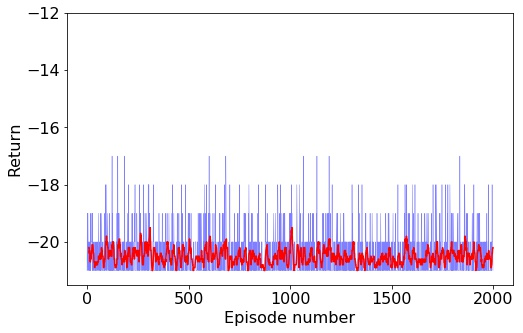
\includegraphics[width=0.4\textheight]{dqn_return.jpeg}\label{fig:DQN-learning}}\\
   	\subfloat[]{
   		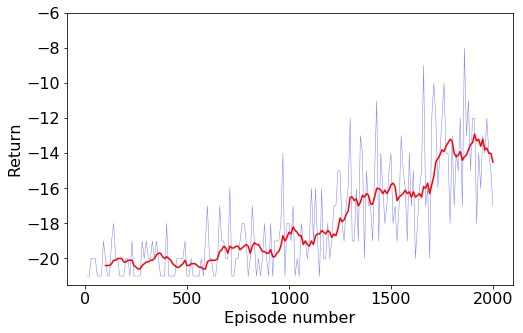
\includegraphics[width=0.4\textheight]{pg_return.jpeg}\label{fig:PG-learning}}
    \caption{Agent training performance for (a) DQN and (b) Policy Gradient algorithm. In blue the return obtained at the end of an episode, and in red the moving average calculated in a window of 10 episodes.}
    \label{fig:Preprocessing}
  \end{center}
\end{figure}
\hl

\section{Conclusion}
\subsection{Reflection and improvement}
Reinforcement learning is a very fascinating field of machine learning, that has recently attracted a lot of attention from the AI community due to the different problems where it could be applied with possibly superior performances of human beings. Although RL algorithms has been developed several years ago, significant results have been obtained only recently by combining them with neural network models. Despite the complexity of understanding and applying these methods, the main difficulty in using deep-RL was that it requires very long computational times. This makes it difficult to test and debug the code when the algorithm is not performing well.\\
An obvious improvement to the current work would be to understand why the DQN algorithm is not performing better that a random agent after a relatively long training time. It would be interesting also to test more advanced version of the algorithms such as Actor-Critic DQN, and a Policy Gradient version that uses the value function together with the the discounted rewards \cite{Mnih2016}. 
  
\hl

\begin{thebibliography}{9}
\bibitem{Mnih2013}  V. Mnih et al. Playing Atari With Deep Reinforcement Learning. \emph{NIPS Deep Learning Workshop}, 2013
\bibitem{Mnih2015}  V. Mnih et al. Human-level control through deep reinforcement learning. \emph{Nature} 518 (7540):529--533, 2013
\bibitem{Mnih2016}  V. Mnih et al. Asynchronous Methods for Deep Reinforcement Learning. \emph{ International Conference on Machine Learning}, 2016
\bibitem{Sutton} R.S. Sutton and A.G. Barto. \emph{Reinforcement Learning: An Introduction}. Second Edition. Complete Draft, 2017
\bibitem{OpenAI} http://gym.openai.com/envs/Pong-v0/
\bibitem{Jaromiru} https://jaromiru.com/2016/10/03/lets-make-a-dqn-implementation/
\bibitem{Williams1992}  R.J. Williams. Simple statistical gradient-following algorithms for connectionist
\bibitem{Karpathy} http://karpathy.github.io/2016/05/31/rl/
\bibitem{Ecoffet} https://becominghuman.ai/lets-build-an-atari-ai-part-1-dqn-df57e8ff3b26

\end{thebibliography}

\end{document}